\providecommand{\main}{..}
\documentclass[\main/TL_liquid.tex]{subfiles}
\graphicspath{{\main/images/}}
\begin{document}
\section{分割と母関数}
\begin{frame}{分割数}
    \begin{block}{分割数}
        自然数$N$を非増加の自然数列$\lambda_1\ge\lambda_2\ge\cdots\ge\lambda_n$によって
        \begin{align}
            N = \lambda_1 + \lambda_2 + \cdots + \lambda_n
        \end{align}
        と表せるとき、$(\lambda_1,\ldots,\lambda_n)$を$N$の分割と呼ぶ。
        $N$に対してあり得る分割の総数を$p(N)$と書き、$N$の分割数という。
    \end{block}
    小さい$N$に対して、
    \begin{align*}
        p(1) = 1,
        \\
        p(2) = 2,
        \\
        p(3) = 3,
        \\
        p(4) = 5.
    \end{align*}
\end{frame}

\begin{frame}{ボソン系の分配関数と分割数}
    エネルギー準位が$\epsilon,2\epsilon,3\epsilon,\ldots$であるような、
    相互作用しないボソン系を考えよう。
    具体的には、以下のハミルトニアンを考える。
    \begin{align}
        H = \sum_{k=1}^\infty k\epsilon n_k
    \end{align}
    $n_k$は準位$k$にいるボソンの粒子数である。系の大分配関数は、
    \begin{align}
        q = e^{-\beta\epsilon}
    \end{align}
    とおくことで、
    \begin{align}
        \Xi(\beta,0)
        = \prod_{k=1}^\infty \sum_{n_k=0}^\infty q^{kn_k}
        = \prod_{k=1}^\infty \frac{1}{1-q^k}
    \end{align}
    と表される。
    ただし、化学ポテンシャルは$0$とした。
\end{frame}

\begin{frame}{ボソン系の分配関数と分割数}
    ここで、系のエネルギーを$E = N\epsilon$と固定すると、
    系が取りうる状態の数は$N$の分割数$p(N)$に一致する。
    したがって、
    \begin{align}
        \Xi(\beta,0)
        = \sum_{N=1}^\infty p(N)q^N
    \end{align}
    と書ける。
    ここから、分割数の母関数に対する恒等式
    \begin{align}
        \sum_{N=1}^\infty p(N)q^N
        = \prod_{k=1}^\infty \frac{1}{1-q^k}
    \end{align}
    を得る。
\end{frame}

\begin{frame}{Young図形}
    例えば
    $
        9 = 4+3+1+1
    $
    であるが、これを以下のような箱を並べた図形で表す。
    \begin{figure}[H]
        \centering
        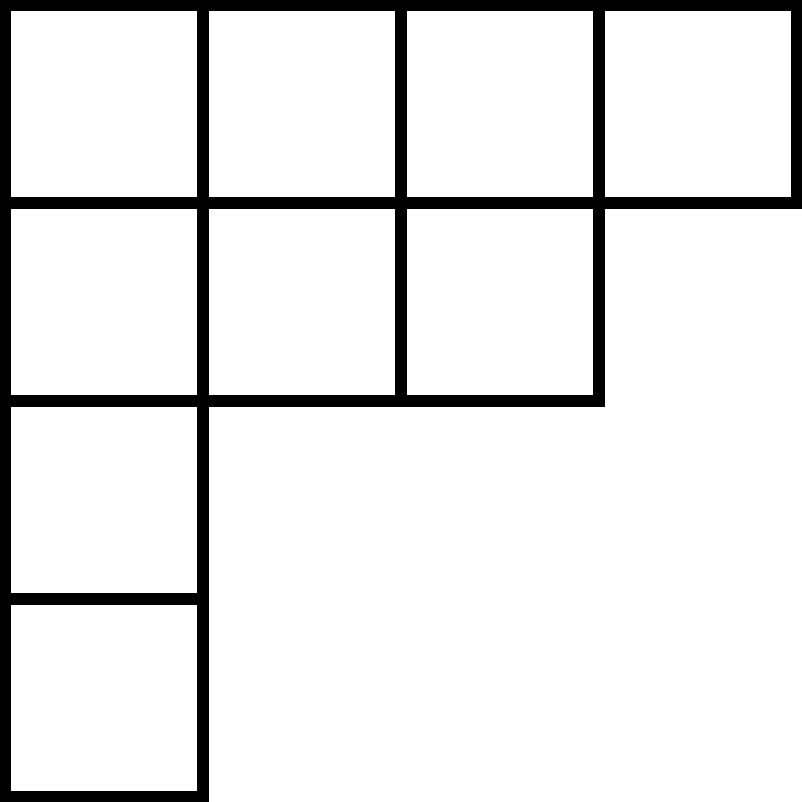
\includegraphics[scale = 0.15]{Young.pdf}
    \end{figure}
    このような図形をYoung図形と呼ぶ。
\end{frame}

% \begin{frame}{共役な分割}
%     分割を拡張して、制限付きの分割を考えよう。
%     例えば、分割する個数を3個以内にするという制限をつけてみよう。
%     このとき、$5$は
%     \begin{align}
%         5 = 4+1 = 3+2 = 2+2+1
%     \end{align}
%     の$4$通りに分割できる。一方、$3$以下の数によって分割するという制限をつけると、
%     \begin{align}
%         3+1+1 = 2+2+1 = 2+1+1+1 = 1+1+1+1+1
%     \end{align}
%     の$4$通りに分割できる。
% \end{frame}

\begin{frame}{Eulerの分割恒等式}
    $7$を異なる自然数で分割すると、
    \begin{align}
        7 = 6+1 = 5+2 = 4+3 = 4+2+1
    \end{align}
    の$5$通りである。これをストリクトな分割と呼ぶ。
    一方$7$を奇数のみで分割すると、
    \begin{align}
        7 = 5+2\cdot1 = 2\cdot3+1 = 3+4\cdot1 = 7\cdot1
    \end{align}
    で、この場合も$5$通りである。
    一般の$N$に対し、
    異なる自然数による分割の数を$p_{\mathrm{str}}(N)$、
    奇数による分割の数を$p_{\mathrm{odd}}(N)$とおく。
    実は任意の$N$に対して
    \begin{align}
        p_{\mathrm{str}}(N) = p_{\mathrm{odd}}(N)
    \end{align}
    が成り立つ。これをEulerの分割恒等式と呼ぶ。
\end{frame}

\begin{frame}{Eulerの分割恒等式}
    Eulerの分割恒等式は、分割の間の全単射を構成することで証明される。
    \begin{gather*}
        (7) \leftrightarrow (7)
        \\[10pt]
        (6,1) \leftrightarrow (3,3,1)
        \\[10pt]
        (4,2,1) \leftrightarrow (1,1,1,1,1,1,1)
    \end{gather*}
\end{frame}

\begin{frame}{母関数の恒等式}
    Eulerの分割恒等式を母関数の世界から見てみる。

    ストリクトな分割は、エネルギー準位が$\epsilon,2\epsilon,3\epsilon,\ldots$であるようなフェルミ系に、
    粒子を配置することと等価である。
    この系の分配関数は
    \begin{align}
        \Xi_{\mathrm{F}}(\beta,0)
        = \prod_{k=1}^\infty \sum_{n_k = 0,1} q^{kn_k}
        = \prod_{k=1}^\infty (1+q^k)
    \end{align}
    となる。
    ただし$q = e^{-\beta\epsilon}$である。
    したがって、
    \begin{align}
        \sum_{N=1}^\infty p_{\mathrm{str}}(N)q^N
        = \prod_{k=0}^\infty (1+q^k)
        \label{generating function of strict partition}
    \end{align}
    が成り立つ。
\end{frame}

\begin{frame}{母関数の恒等式}
    奇数による分割は、エネルギー準位が$\epsilon,3\epsilon,5\epsilon,\ldots$であるようなボース系に、
    粒子を配置することと等価である。
    この系の分配関数は$q = e^{-\beta\epsilon}$として、
    \begin{align}
        \Xi_{\mathrm{B}}(\beta,0) = \prod_{k=1}^\infty \sum_{n_k=0}^\infty q^{(2k-1)n_k} = \prod_{k=1}^\infty \frac{1}{1-q^{2k-1}}
    \end{align}
    と計算できるから、
    \begin{align}
        \sum_{N=1}^\infty p_{\mathrm{odd}}(N)q^N = \prod_{k=1}^\infty \frac{1}{1-q^{2k-1}}
        \label{generating function of odd partition}
    \end{align}
    が成り立つ。
\end{frame}

\begin{frame}{母関数の恒等式}
    (\ref{generating function of strict partition})と
    (\ref{generating function of odd partition})
    を見比べると、
    \begin{align}
        \prod_{k=1}^\infty (1+q^k)
        =
        \prod_{k=1}^\infty \frac{1}{1-q^{2k-1}}
    \end{align}
    を得る。これは以下のように直接示すことができる。
    \begin{align}
        \prod_{k=1}^\infty (1+q^k)
        & \nonumber
        = \prod_{k=1}^\infty \frac{1-q^{2k}}{1-q^k}
        \\ & \nonumber
        = \prod_{k=1}^\infty \frac{1-q^{2k}}{(1-q^{2k})(1-q^{2k-1})}
        \\ &
        = \prod_{k=1}^\infty \frac{1}{1-q^{2k-1}}
    \end{align}
\end{frame}
\end{document}